\Exercise[title={Integral delimitada entre funcions}]

%\begin{Exercise}[label=Ex7]

Sigui $R$ la regió delimitada  per les corbes $f(x)=x^2+2x-3$, $g(x)=3x+3$. 
\begin{itemize}
  
  \item Representeu gràficament la regió $R$.
  \item Determineu l'àrea $A(R)$ de la regió $R$.
  \item Calculeu $\int \int_R x dxdy$ .
\end{itemize}


%\end{Exercise}

\Answer

%  \begin{Answer}[ref=Ex7]
\begin{itemize}
  \item 
Comencem per dibuixar les dues funcions.

    \begin{center}
      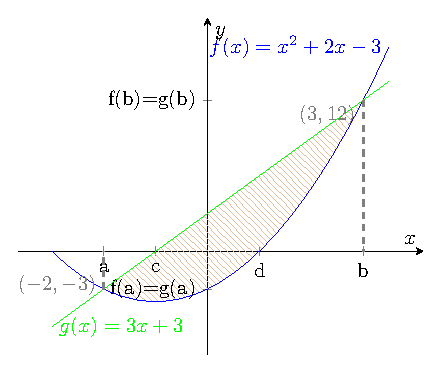
\includegraphics[width=0.5\textwidth]{areax2plus2xminus33xplus3.pdf}
    \end{center}

A partir de solucionar 
\[
  x^2+2x-3=3x+3
\]
trobem que es tallen en els punts $(-2,-3)$ i $(3,12)$.

\item Per trobar l'àrea podem pensar en dividir el càlcul en tres parts, 
si ens fan dubtar els signes de les funcions:

\[
  A(R)=\int_a^c [f(x)-g(x)] dx +  \int_c^d [g(x)+f(x)] dx + \int_d^b [g(x)-f(x)] dx
\]

o bé, més pràctic, podem sumar un valor superior a 4 a les dues funcions per tal que ens quedin les dues damunt de l'eix de les abscisses.\footnote{Només cal trobar el mínim de la funció parabòlica que es dona quan $f'(x)=2x+2=0$, que passa a $x=-1$, on $f(x)=-4$.}
Per tant, l'àrea serà igual a
\[
  A(R) = \int_a^b [(g(x)+4)-(f(x)+4)] dx = \int_a^b [g(x)-f(x)] dx 
  \] 
  \[
    A(R) = \int_{-2}^{3} [(3x+3)-(x^2+2x-3)] dx =  \int_{-2}^{3} [-x^2+x+6] dx = \left[-\frac{x^3}{3}+\frac{x^2}{2}+6x\right]_{-2}^3= \frac{125}{6}
    \] 
  
\item Com que ens donen dues funcions de la variable $x$, el més pràctic és integrar primer respecte $y$ i despreś respecte $x$:

\begin{eqnarray*}
V=\int \int_R x dx dy &=& \int \int_R x dy dx\\
&=& \int_{x=-2}^{x=3} \left[ \int_{x^2+2x-3}^{3x+3} x dy \right]dx  \\
&=& \int_{x=-2}^{x=3} x [(3x+3)-(x^2+2x-3)] dx \\
&=& \left[-\frac{x^4}{4}+\frac{x^3}{3}+3x^2\right]_{-2}^3\\
&=& \left(-\frac{3^4}{4}+\frac{3^3}{3}+3^3\right)-\left(-\frac{(-2)^4}{4}+\frac{(-2)^3}{3}+3 (-2)^2\right)
=\frac{125}{12}
\end{eqnarray*}
\end{itemize}


%\end{Answer}
